\title{Parquet}
\titlerunning{Parquet}
\author{Silvan Heller}
\authorrunning{S. Heller}

\institute{University of Basel \\ \coursename\ (\courseacronym) course \\ \semesterCapitals} % Please do NOT change this line.
\maketitle



\section*{HOW TO}
This template is used for the workshop reports of the \coursename\ course. Remove this section by editing the \texttt{reportContent.tex} file \textbf{after} you have understood how to use this template.

\subsection*{Folder Structure}
\begin{lstlisting}[escapechar=!]
WorkshopReport /
  |- reportContent /  <-- YOUR working folder
      |- images /     <-- Images are stored here
      |- sections /   <-- Additional sections / tex-files here
          |- _HOWTO_.tex    <-- *this* How To section
          |- introduction.tex
          |- lessons-learned.tex
          '- section2.tex
      '- reportContent.tex  <-- Change your section imports here
  |- !\rootDocument!  <-- DO NOT alter this file
  |- llncs.cls                            <-- NOR that
  |- splncs03.bst                         <-- NOR that
  '- UniBas_Logo_EN_Schwarz_RGB_65.pdf    <-- NOR that
\end{lstlisting}
\ 

\subsection*{Setup}
Your report is compiled using the \texttt{\rootDocument} file. Therefore, we suggest that you set the file \texttt{\rootDocument} as the Master-/Root-Document that you can conveniently work on your report. 


\subsection*{Images}
Images placed in the \texttt{images} sub-folder can be used directly in the \texttt{\textbackslash includegraphics} command -- see also \Cref{fig:rosette}. Also, sub-figures are possible: \Cref{fig:fly,fig:flies}.

Please \textsc{do~not} store your images elsewhere! 

\begin{figure}[tb]
\centering
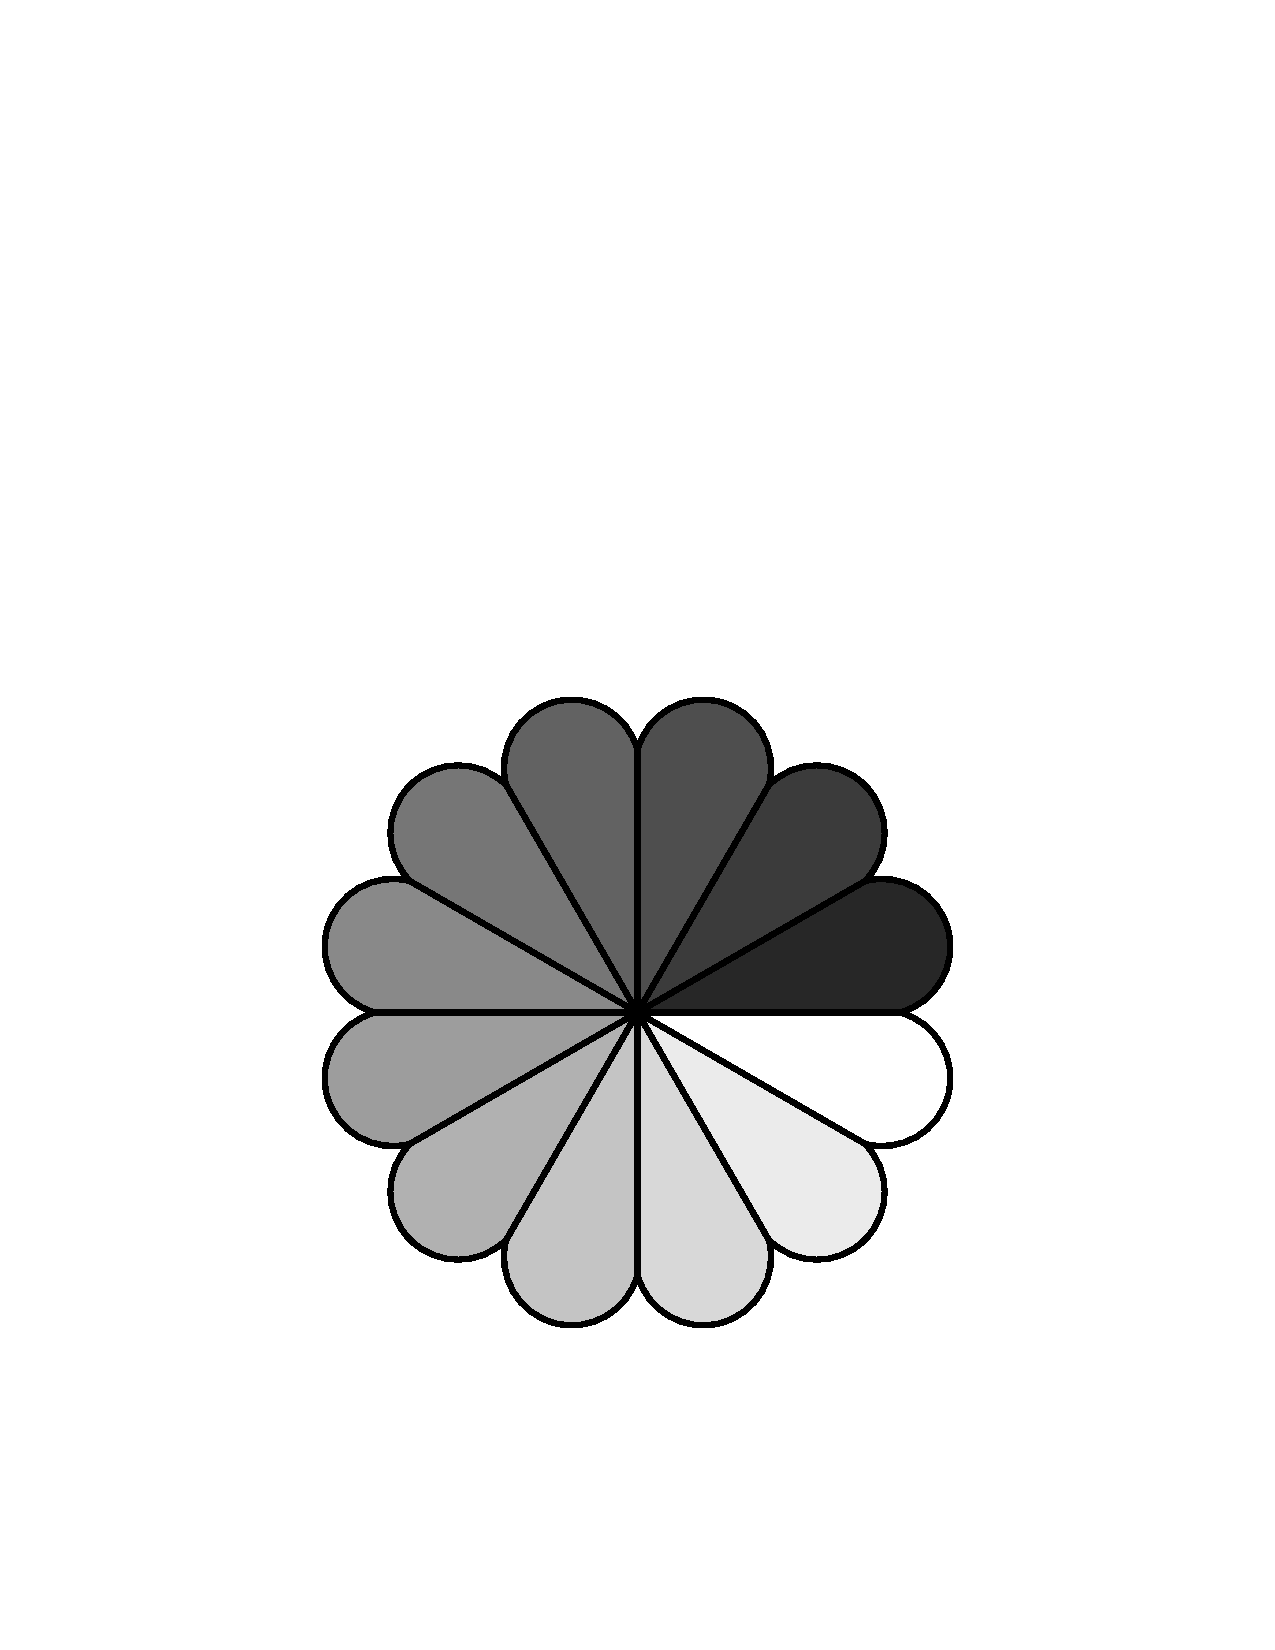
\includegraphics[width=0.45\textwidth]{rosette}
\caption{Example figure stored in the \texttt{images} sub-folder and displayed with \texttt{\textbackslash includegraphics[width=0.45\textbackslash textwidth]\{rosette\}}}
\label{fig:rosette}
\end{figure}

\begin{figure}[tb]
\centering
    %\subfloat[CAPTION]{BILDERCODE}\qquad
    \subfloat[A fly\label{fig:fly}]{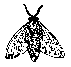
\includegraphics[width=0.4\textwidth]{fly}}\qquad
    \subfloat[Flies\label{fig:flies}]{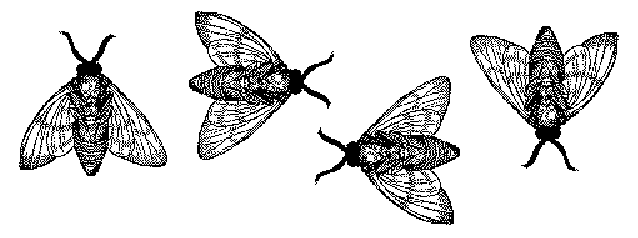
\includegraphics[width=0.45\textwidth]{flies}}
\caption{Example figure stored in the \texttt{images} sub-folder}
\label{fig:example subfigure}
\end{figure}


\subsection*{Code}
To illustrate code use the \texttt{lstlisting} environment:
\begin{lstlisting}[language=Java]
public void foo( final int bar ) {
  System.out.println( bar );
}
\end{lstlisting}


\subsection*{References}
Your references are stored in the \texttt{reportContent.tex} file and used with the \texttt{\textbackslash cite} command. For example: \cite{IEEEhowto:kopka}.

Unfortunately, you cannot use a bibliography generated by BibTeX as a .bbl file directly. Use \texttt{\textbackslash bibliographystyle\{IEEEtran\}} and \texttt{\textbackslash bibliography\{references\}} (the argument is your BibTeX string definitions and bibliography database(s), e.\,g. \texttt{references.bib}) along with all \texttt{\textbackslash cite} commands in a separate \texttt{tex} document to generate a .bbl file using BibTeX. Then, copy manually the resultant .bbl file content into the \texttt{thebibliography} environment in the \texttt{reportContent.tex} file. Also, set the second argument of the \texttt{\textbackslash begin} to the number of references (used to reserve space for the reference number labels box).

\pagebreak % TODO: Comment this line AFTER you have understood how to use this template



\section{Introduction} \label{sec:introduction}

As datasets grow, so does the need for storing them efficiently and in a format that is suited to the needs of high-volume, high-velocity and high-variety data.
In this Workshop report, we will discuss Parquet\footnote{https://parquet.apache.org/} as an example of a file format suited for 'Big Data'.

\subsection{History}
Google outlined in 2010 how they were using Dremel \cite{dremel:melnik} and the Dremel file format to store high-variety structured data at petabyte scale in a columnar format.
Since Dremel is, as most Google tools are, proprietary and not open source,
Twitter and Cloudera started the Apache Parquet project as an open source implementation \cite{parquet-announcement:kestelyn}.
The goal was to provide an efficient columnar storage format for the Hadoop ecosystem.
Today, Parquet is used in production at multiple companies, the most notable ones being Stripe and Twitter \cite{adopters:parquet}.

\subsection{Using Parquet}
Since Parquet is a file format, it requires implementation and tools around it.
We have used Apache Spark \cite{spark:zaharia}, which has built-in support for Parquet and other file formats and is thus ideal to compare Parquet fairly.
The application implemented is a benchmark to compare Parquet, JSON, CSV and Apache ORC\footnote{https://orc.apache.org/}.
Our benchmark will contain two scenarios, one with a table which has a lot of columns but the queries used only access one column and the other one with nested objects.

\subsection{Outline}
Chapter \ref{sec:parquet} will describe the Parquet format in detail.
To see how Parquet compares to other data storage formats, Chapter \ref{sec:application} outlines two scenarios which will be used to benchmark Parquet.
Chapter \ref{sec:results} contains the benchmark results and Chapter \ref{sec:lessons_learned} concludes with the lessons learned.
\section{Section 2}


\lipsum[1-2] % TODO: DELETE ME (\lipsum[1-2])


\section{Application} \label{sec:application}
In this section, we will cover the implemented benchmark application in detail.
The code is available on Github\footnote{https://github.com/silvanheller/parquet-demo}

\subsection{Technologies used}
Our benchmarking application uses Apache Spark\footnote{http://spark.apache.org/} as Queryengine.
The programming language used is Scala\footnote{https://www.scala-lang.org/}.
We compare Parquet to JSON, CSV and Apache ORC\footnote{https://orc.apache.org/}

\subsection{Scenario I - Column Storage}
\label{sec:scenario-one}
Scenario I is intended to showcase the power of columnar storage formats.
It features a table schema with a lot of columns, only one of which is accessed for the given query.
The other columns are filled with strings, given that today's data sets often feature highly varied and unstructured data.

\subsubsection{Table Layout}
Given a number of rows $n_rows$, a number of columns $n_cols$ and the length of a string $s_length$, the table schema is depicted in Table \ref{table:schema-one}
\begin{table}[h]
\centering
\caption{Table Layout for Scenario 1}
\label{table:schema-one}
\renewcommand{\arraystretch}{1.4}
{\setlength{\tabcolsep}{1em}
\begin{tabular}{|c|c|c|c|c|}
\hline
id      & data1                & data2                & ... & data{[}n\_cols{]}    \\ \hline
1       & rand\_string(s\_len) & rand\_string(s\_len) & ... & rand\_string(s\_len) \\ \hline
...     & ...                  & ...                  & ... & ...                  \\ \hline
n\_rows & rand\_string(s\_len) & rand\_string(s\_len) & ... & rand\_string(s\_len) \\ \hline
\end{tabular}}
\end{table}

\subsubsection{Query}
\label{sec:query-one}
The query we have chosen for this scenario is a simple average over the 'id' column.
Code-snippet \ref{code:scenario1-avg-spark} shows how this is done in Scala and snippet \ref{code:scenario1-avg-sql} shows the equivalent SQL query.
\begin{lstlisting}[language=Scala,caption=Average over the ID Column in Spark, label=code:scenario1-avg-spark, captionpos=b]
def getAVG(df: DataFrame): DataFrame = {
  df.agg(avg("id"))
}
\end{lstlisting}
\begin{lstlisting}[language=SQL,caption=Equivalent SQL Query, label=code:scenario1-avg-sql, captionpos=b]
  SELECT AVG(id) FROM table;
\end{lstlisting}
This requires acessing all rows and prevents automatically created index structures such as in ORC from interfering with our measurements.
Apache Spark uses lazy evaluation for queries, which enables us to read the data from cold storage.
This also means queries are run only once on the dataset since afterwards the data might be cached somewhere.

\subsection{Scenario II - Nested Object Storage}
Scenario II is designed to benchmark nested object storage.
As discussed in Section \ref{section:parquet-nested}, parquet stores nested objects by creating separate tables per attribute.

\subsubsection{Table Layout}

Our Table is a collection of $Persons$. Each Person has a name and an age, two Parents, which in turn have Parents (Four Grandparents).
Each Grandparent is a successor of Adam (inspired by Christian Mythology). Graphically, our Schema is represented in Figure \ref{fig:schema-scenario2}

\begin{figure}[h]
\centering
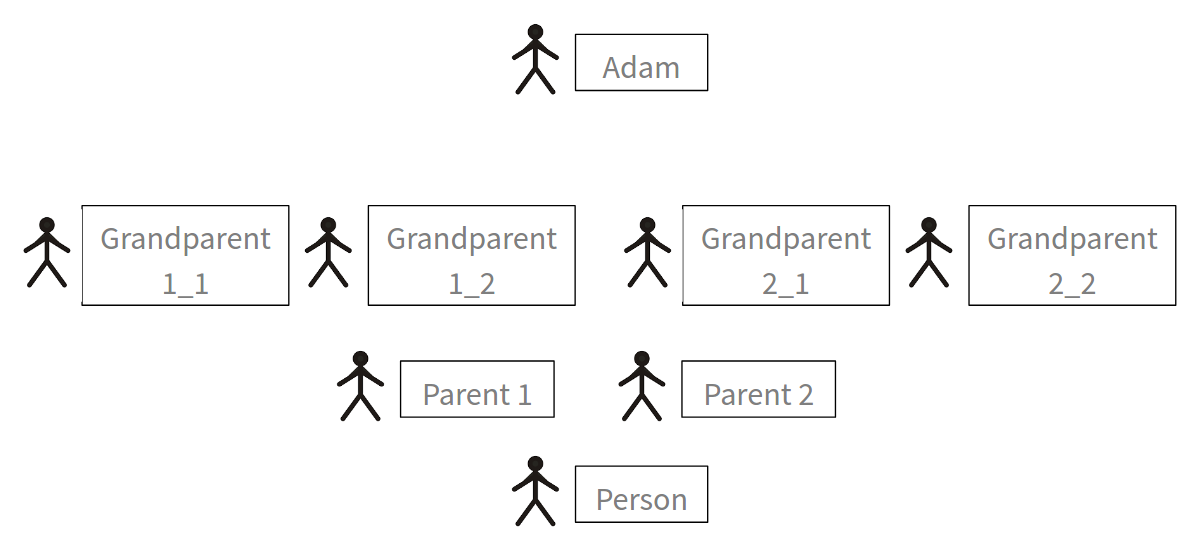
\includegraphics[width=0.8\textwidth]{schema-scenario2.png}
\caption{Scenario 2 visualized}
\label{fig:schema-scenario2}
\end{figure}

For Parquet, this results in 2 (person-columns)+ 4 (parent-columns) + 8 (grandparent-columns) + 8 (adam-columns) = 22 tables.
In the interest of readability, we will not list them all.
%They are: \\
%$person.name$, $person.age$, \\
%$person.parent1.name$, $person.parent1.age$, \,$person.parent2.name$,\, $person.parent2.age$, \\
%$person.parent1.grandparent1_1.name$, $person.parent1.grandparent1_1.age$, $person.parent1.grandparent1_2.name$, $person.parent1.grandparent1_2.age$, \\
%$person.parent2.grandparent2_1.name$, $person.parent2.grandparent2_1.age$, $person.parent2.grandparent2_2.name$, $person.parent2.grandparent2_2.age$, \\
%$person.parent1.grandparent1_1.adam.name$, $person.parent1.grandparent1_1.adam.age$, $person.parent1.grandparent1_2.adam.name$, $person.parent1.grandparent1_2.adam.age$, \\
%$person.parent2.grandparent2_1.adam.name$, $person.parent2.grandparent2_1.adam.age$, $person.parent2.grandparent2_2.adam.name$, $person.parent2.grandparent2_2.adam.age$, \\
\subsubsection{Queries}

Again, we average over a column. This time, we have chosen the $person.parent1.grandparent1\_1.adam$ column.

Code-snippet \ref{code:scenario1-avg-spark} shows how this is done in Scala and snippet \ref{code:scenario1-avg-sql} shows the equivalent SQL query.
\begin{lstlisting}[language=Scala,caption=Average over the ID Column in Spark, label=code:scenario1-avg-spark, captionpos=b]
def getAVG(df: DataFrame): DataFrame = {
  df.agg(avg("parent1.grandparent1_1.adam.age").as("adamage"))
}
\end{lstlisting}
\begin{lstlisting}[language=SQL,caption=Equivalent SQL Query, label=code:scenario1-avg-sql, captionpos=b]
  SELECT AVG(parent1.grandparent1_1.adam.age) FROM table;
\end{lstlisting}

The same considerations as with Scenario I apply when choosing the query.
\section{Results} \label{sec:results}


\subsection{Setup}
We use a local setup of spark since we are interested in I/O speed and not in distribution.
Benchmarks are performed on an Intel i7-3820QM with 12GB RAM. The disk used was a HDD.
\subsection{Scenario I}
\subsubsection{Writing Data}
In Figure \ref{fig:write-one}, we show write time for one million rows and a varying number of columns.
\begin{figure}[!htb]
\caption{Writing Time for Scenario I}
\centering
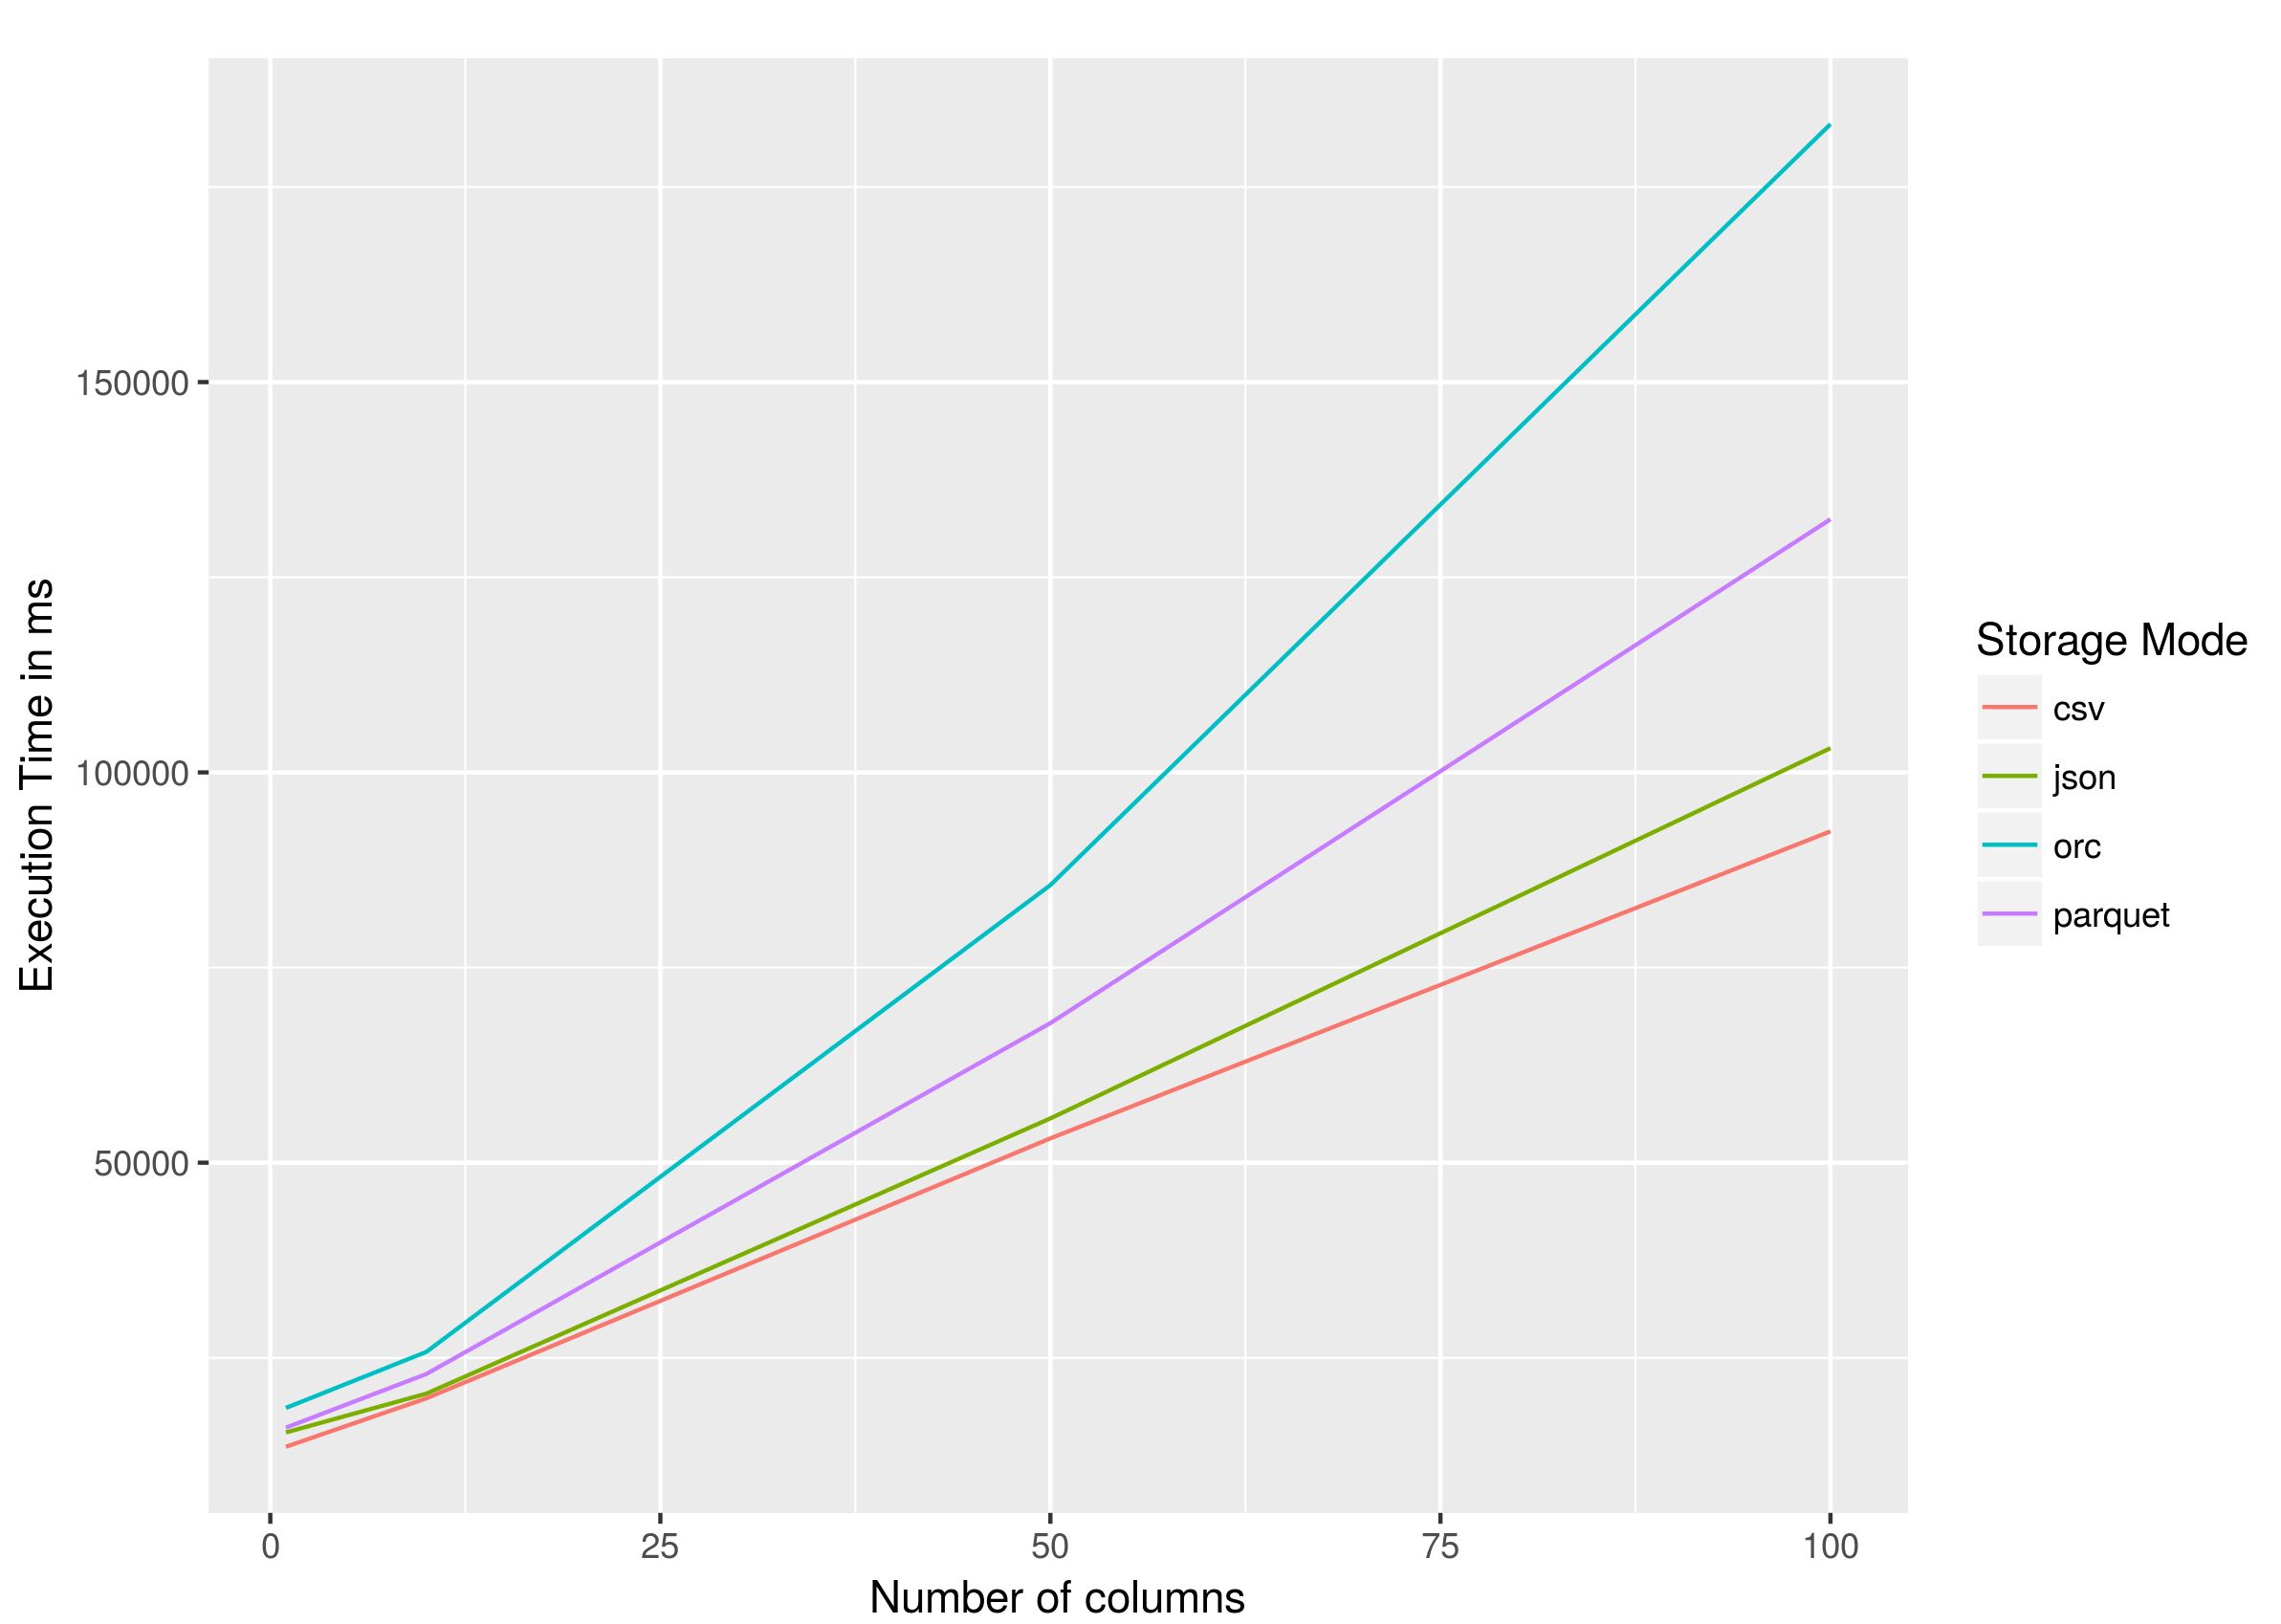
\includegraphics[width=0.75\textwidth]{write-one.png}
\label{fig:write-one}
\end{figure}

As expected, writing csv is fastest since json-files are larger. Parquet being slower is also expected.

\subsubsection{File size}
As expected, JSON uses the most hard disk space with 11 GB (for $10^6$ rows and 100 columns).
Compared with 9.5 GB for ORC, 9.8 GB for Parquet and 9.9 GB for CSV respectively, this is due to the method of schema storage in JSON.
ORC and Parquet perform better as expected since they use compression algorithms to store tables.

\subsubsection{Query}
In Figure \ref{fig:query-one}, we show the execution time of the query described in Section \ref{sec:query-one} for one million rows and a varying number of columns.

\begin{figure}[!htb]
\caption{Query Execution Time for Scenario I}
\centering
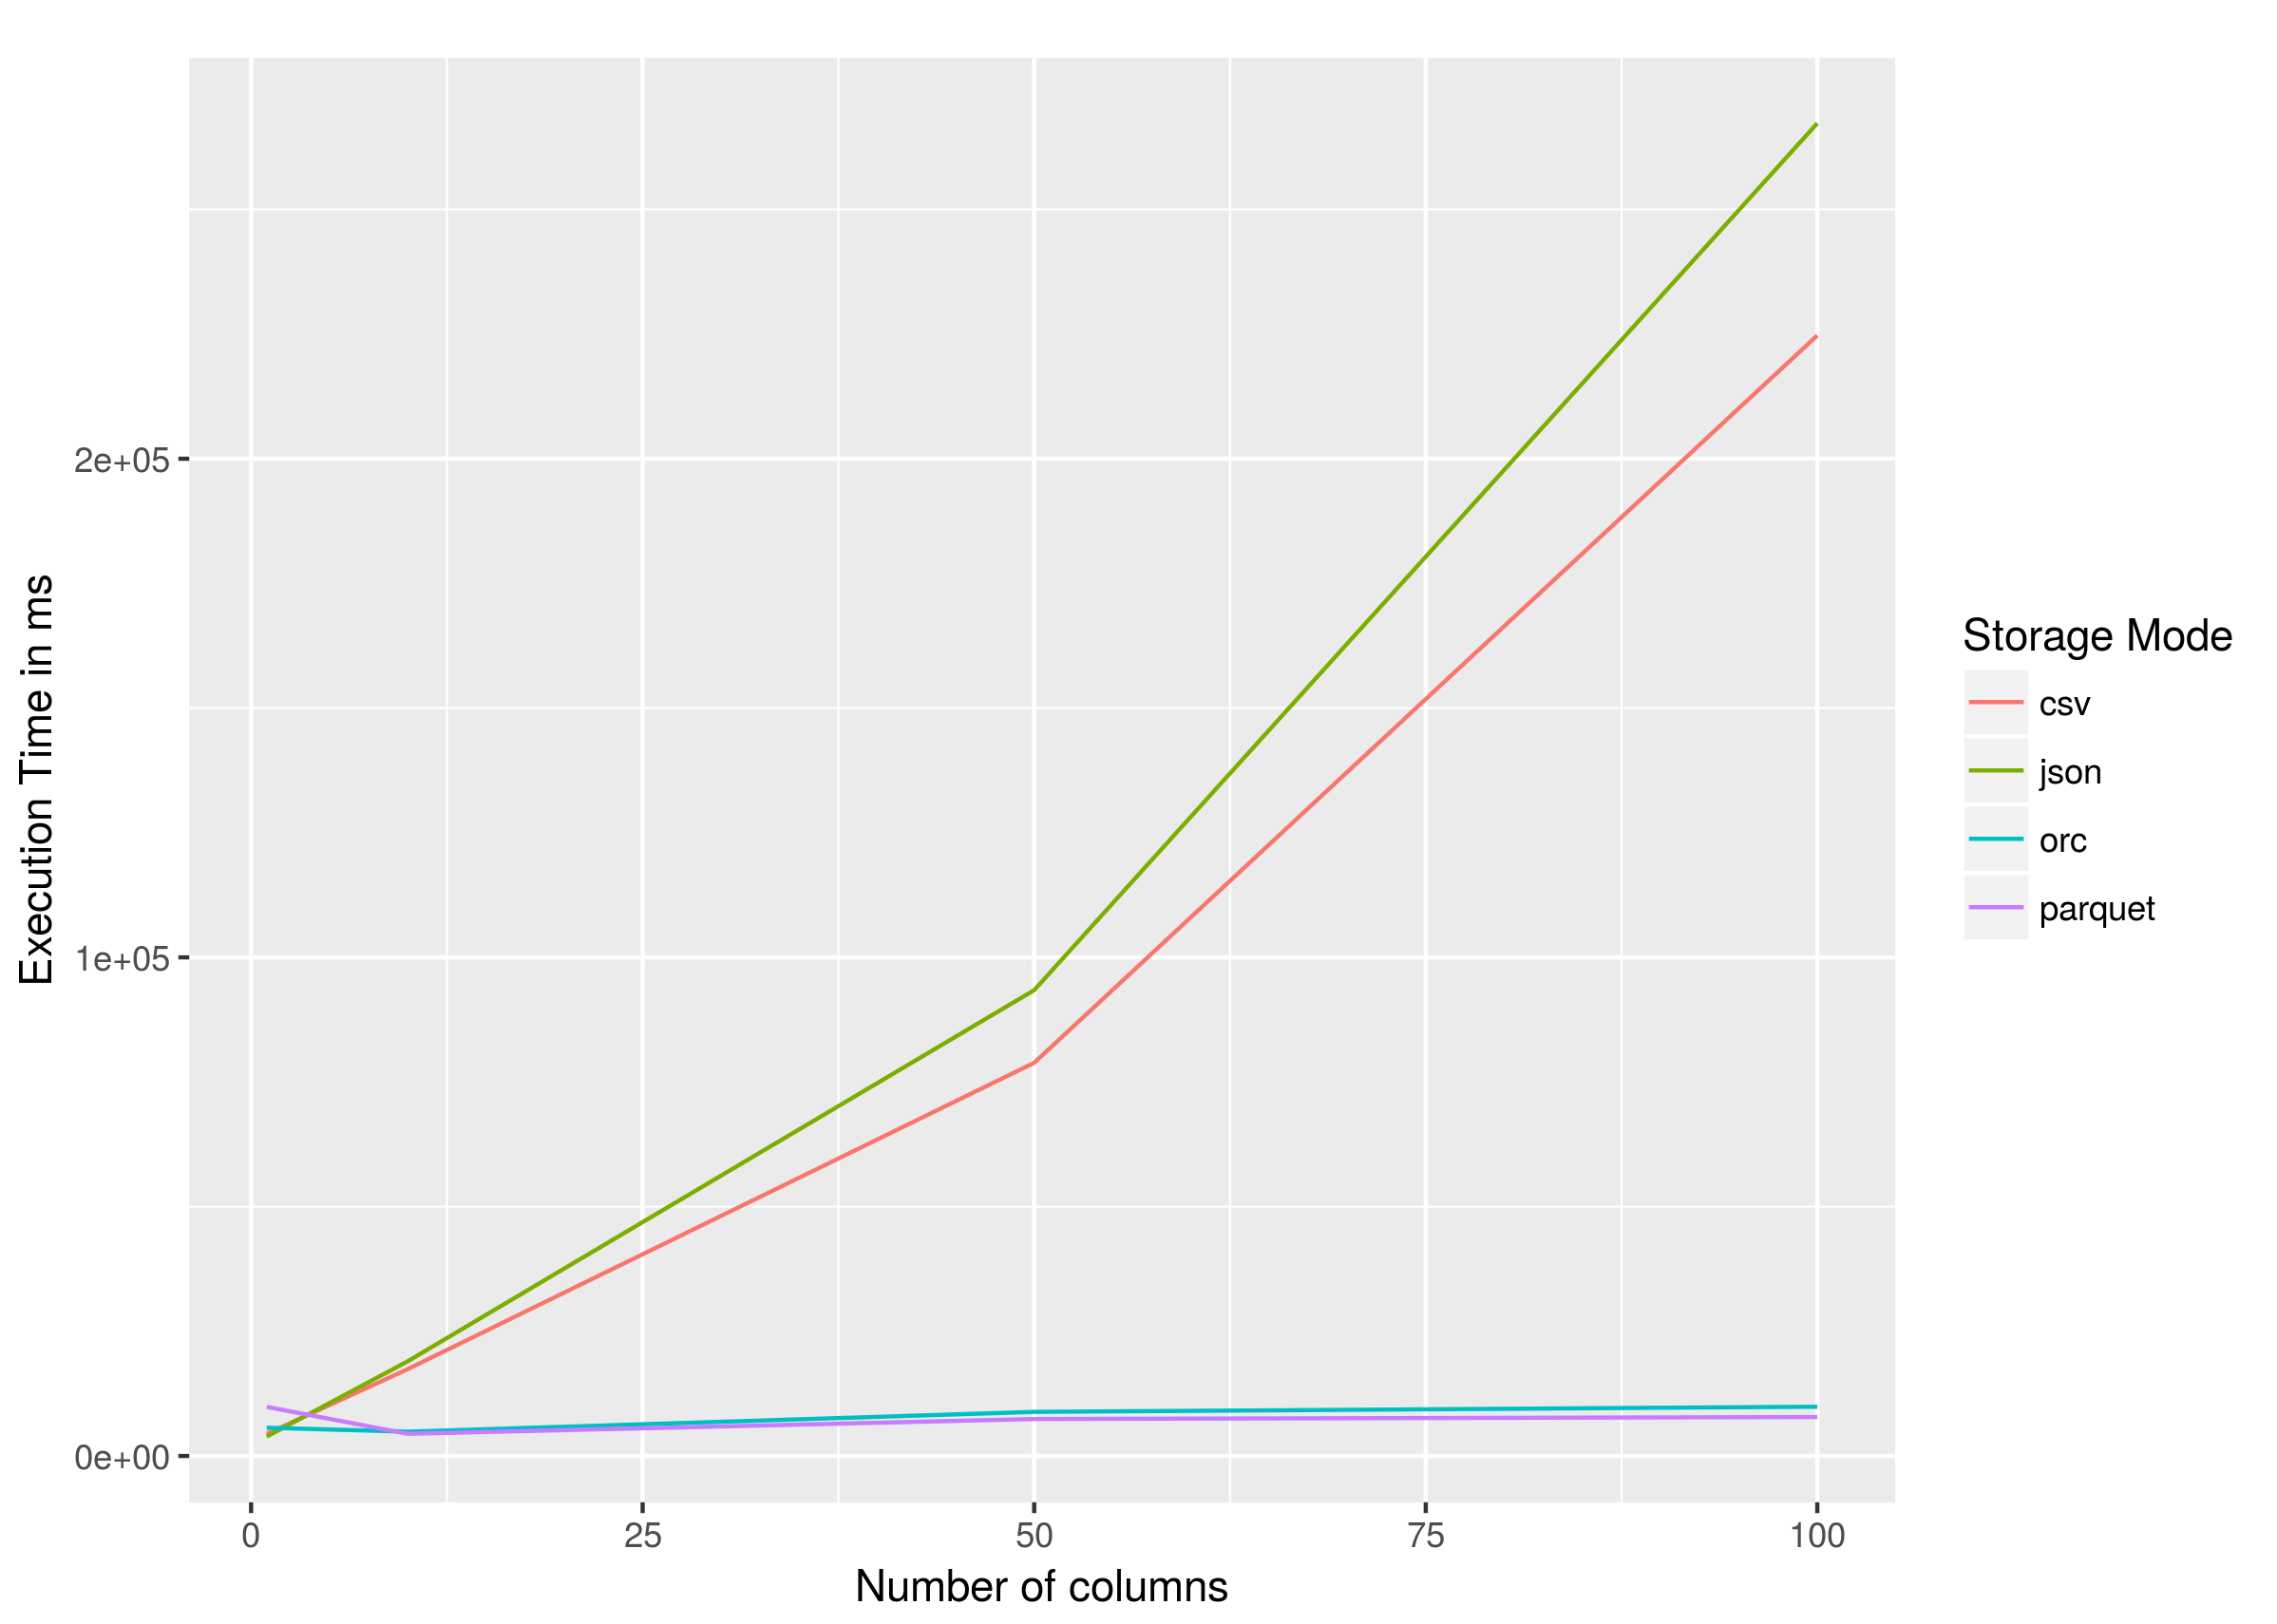
\includegraphics[width=0.75\textwidth]{query-one.png}
\label{fig:query-one}
\end{figure}

As expected, execution time for Parquet is constant as the number of column grows while execution time for JSON and CSV grows linearly.

\subsection{Scenario II}

\subsubsection{Writing Data}
In Figure \ref{fig:write-two}, we show write time for a name length of 50 and a varying number of rows.

\begin{figure}[!htb]
\caption{Writing Time for Scenario II}
\centering
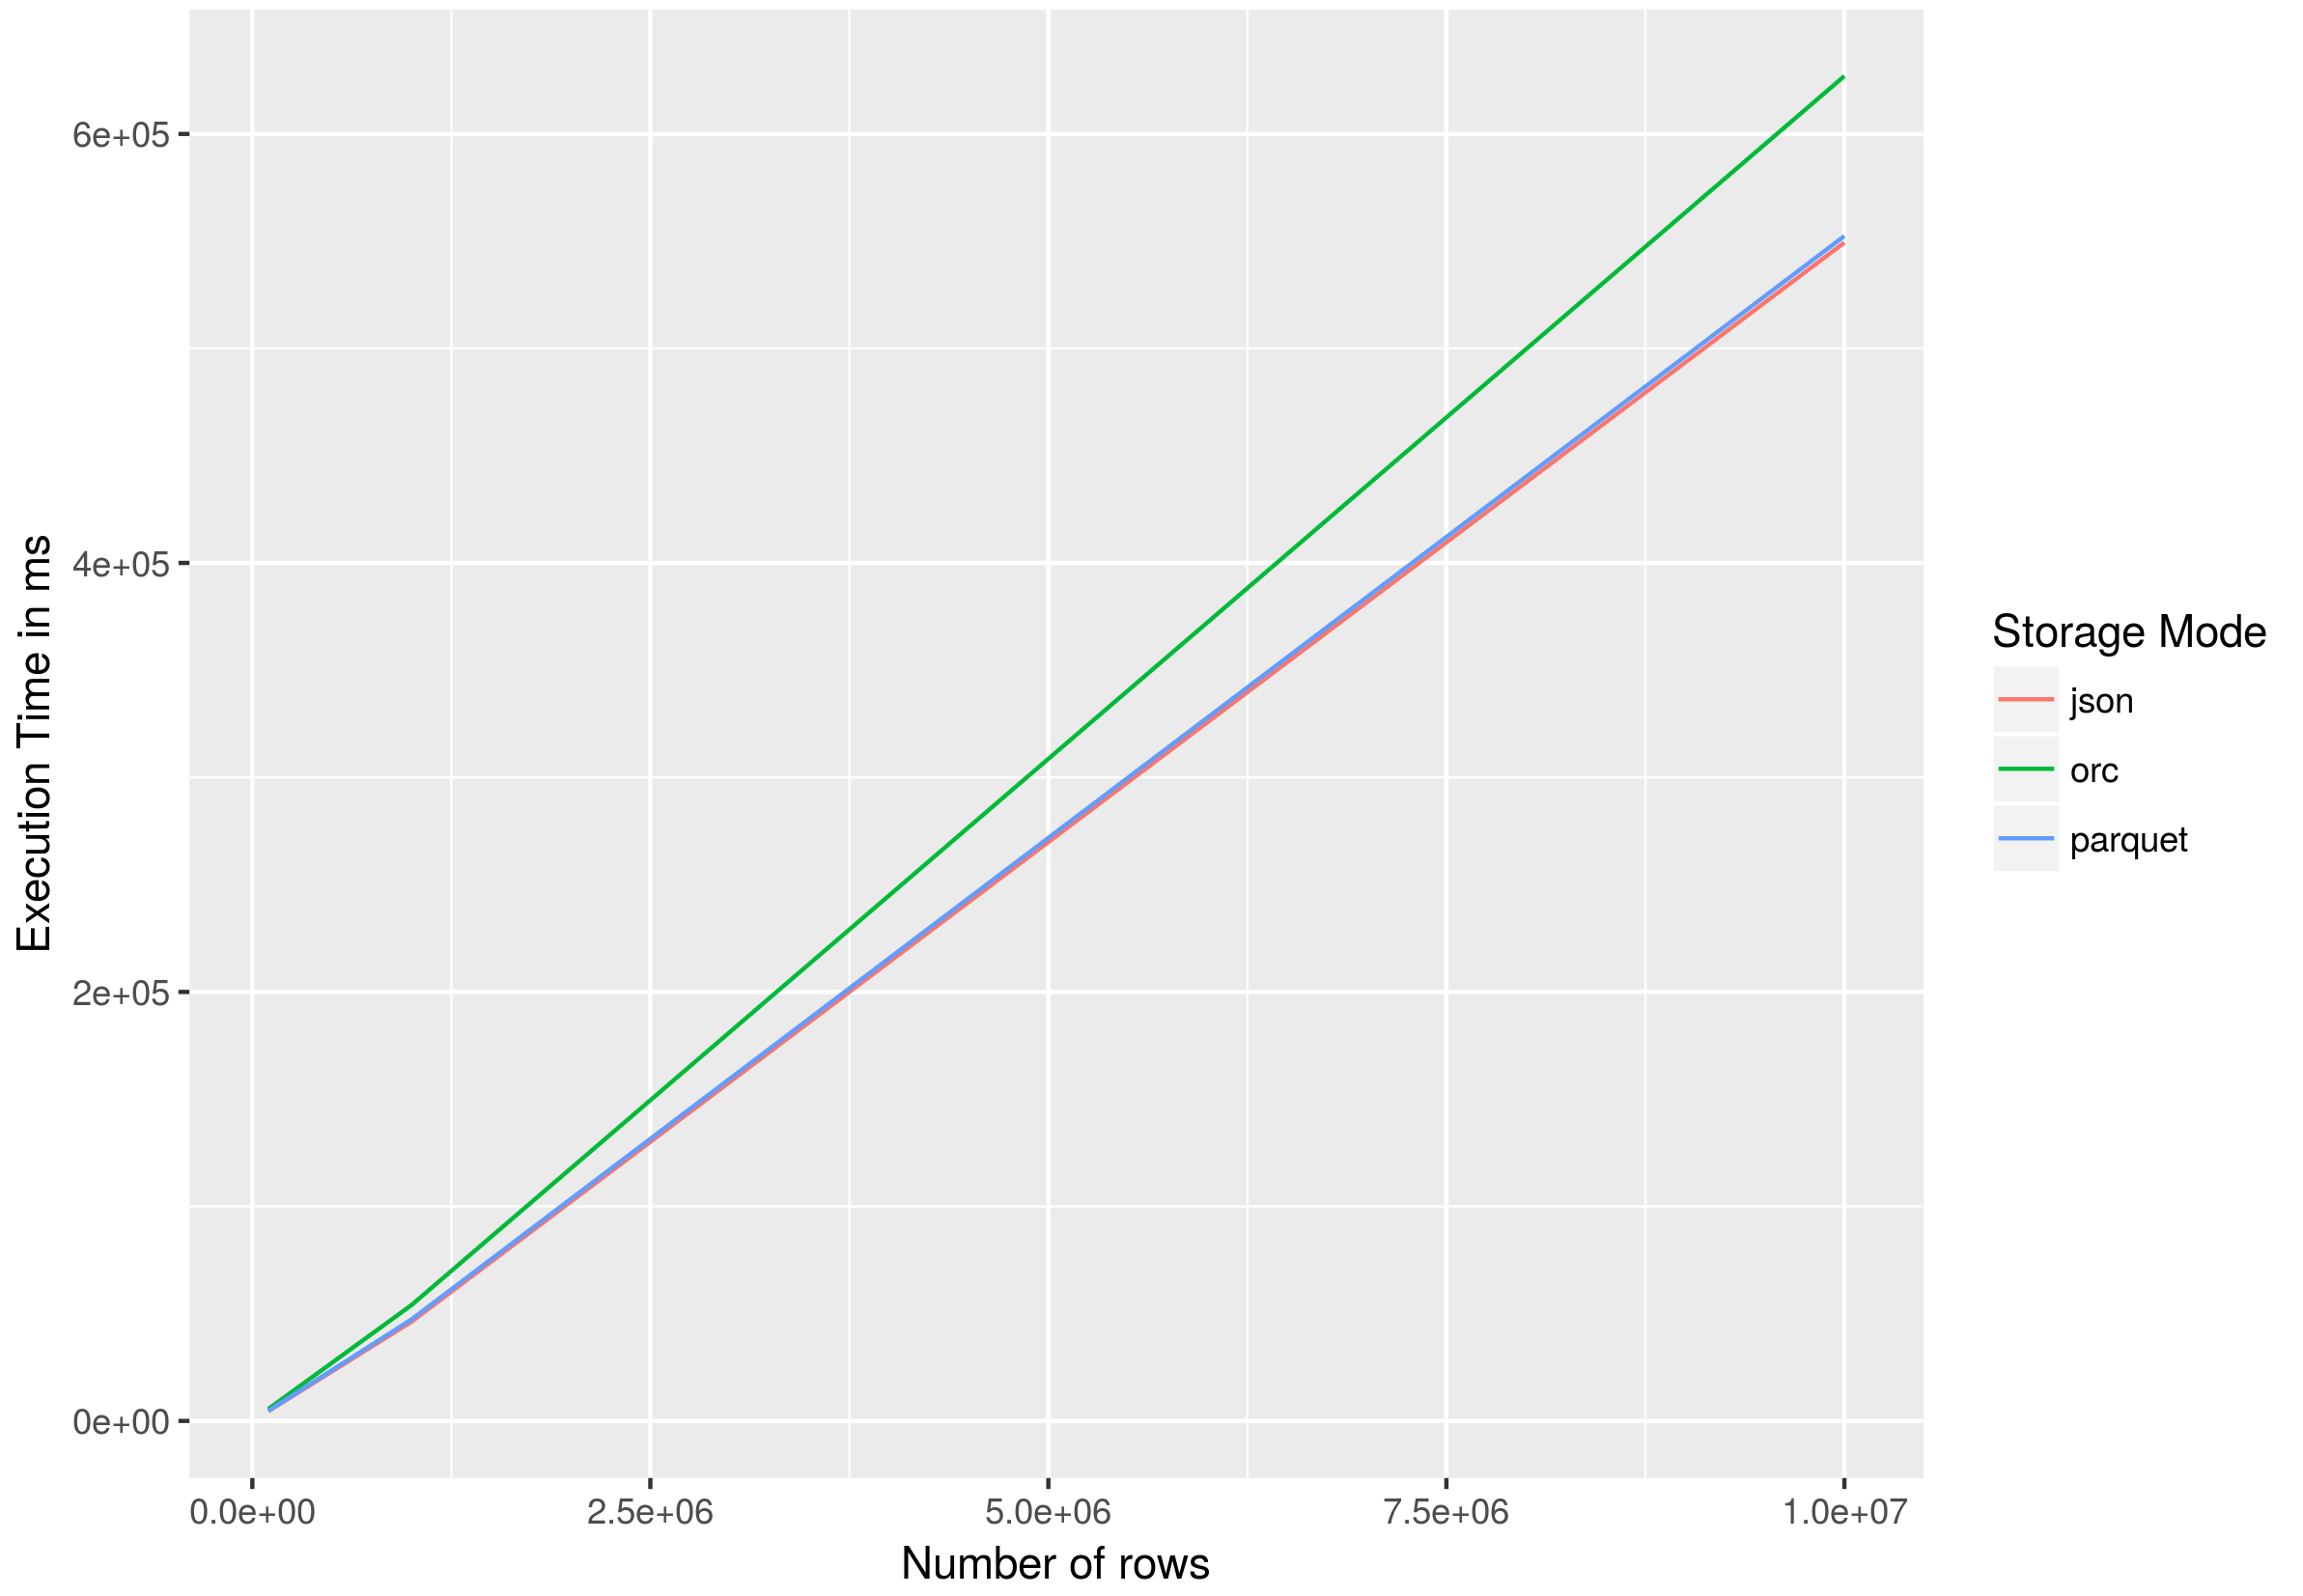
\includegraphics[width=0.75\textwidth]{write-two.png}
\label{fig:write-two}
\end{figure}

For different string lengths, the constant was that Parquet outperforms ORC and is competitive with JSON.
Again, minor write overhead is not the primary concern for most applications.

\subsubsection{File size}
As in Scenario I, JSON uses the most hard disk space with 11 GB (for $10^7$ rows and a name length of 100).
Both compression and the method of storing nested objects pays off for Parquet here as the file size is only 7.0 GB.
ORC sees similar gains and uses 6.7 GB.

\subsubsection{Query}
In Figure \ref{fig:query-two}, we show the execution time of the query described in Section \ref{sec:query-two} for a varying number of rows.

\begin{figure}[!htb]
\caption{Query Execution Time for Scenario II}
\centering
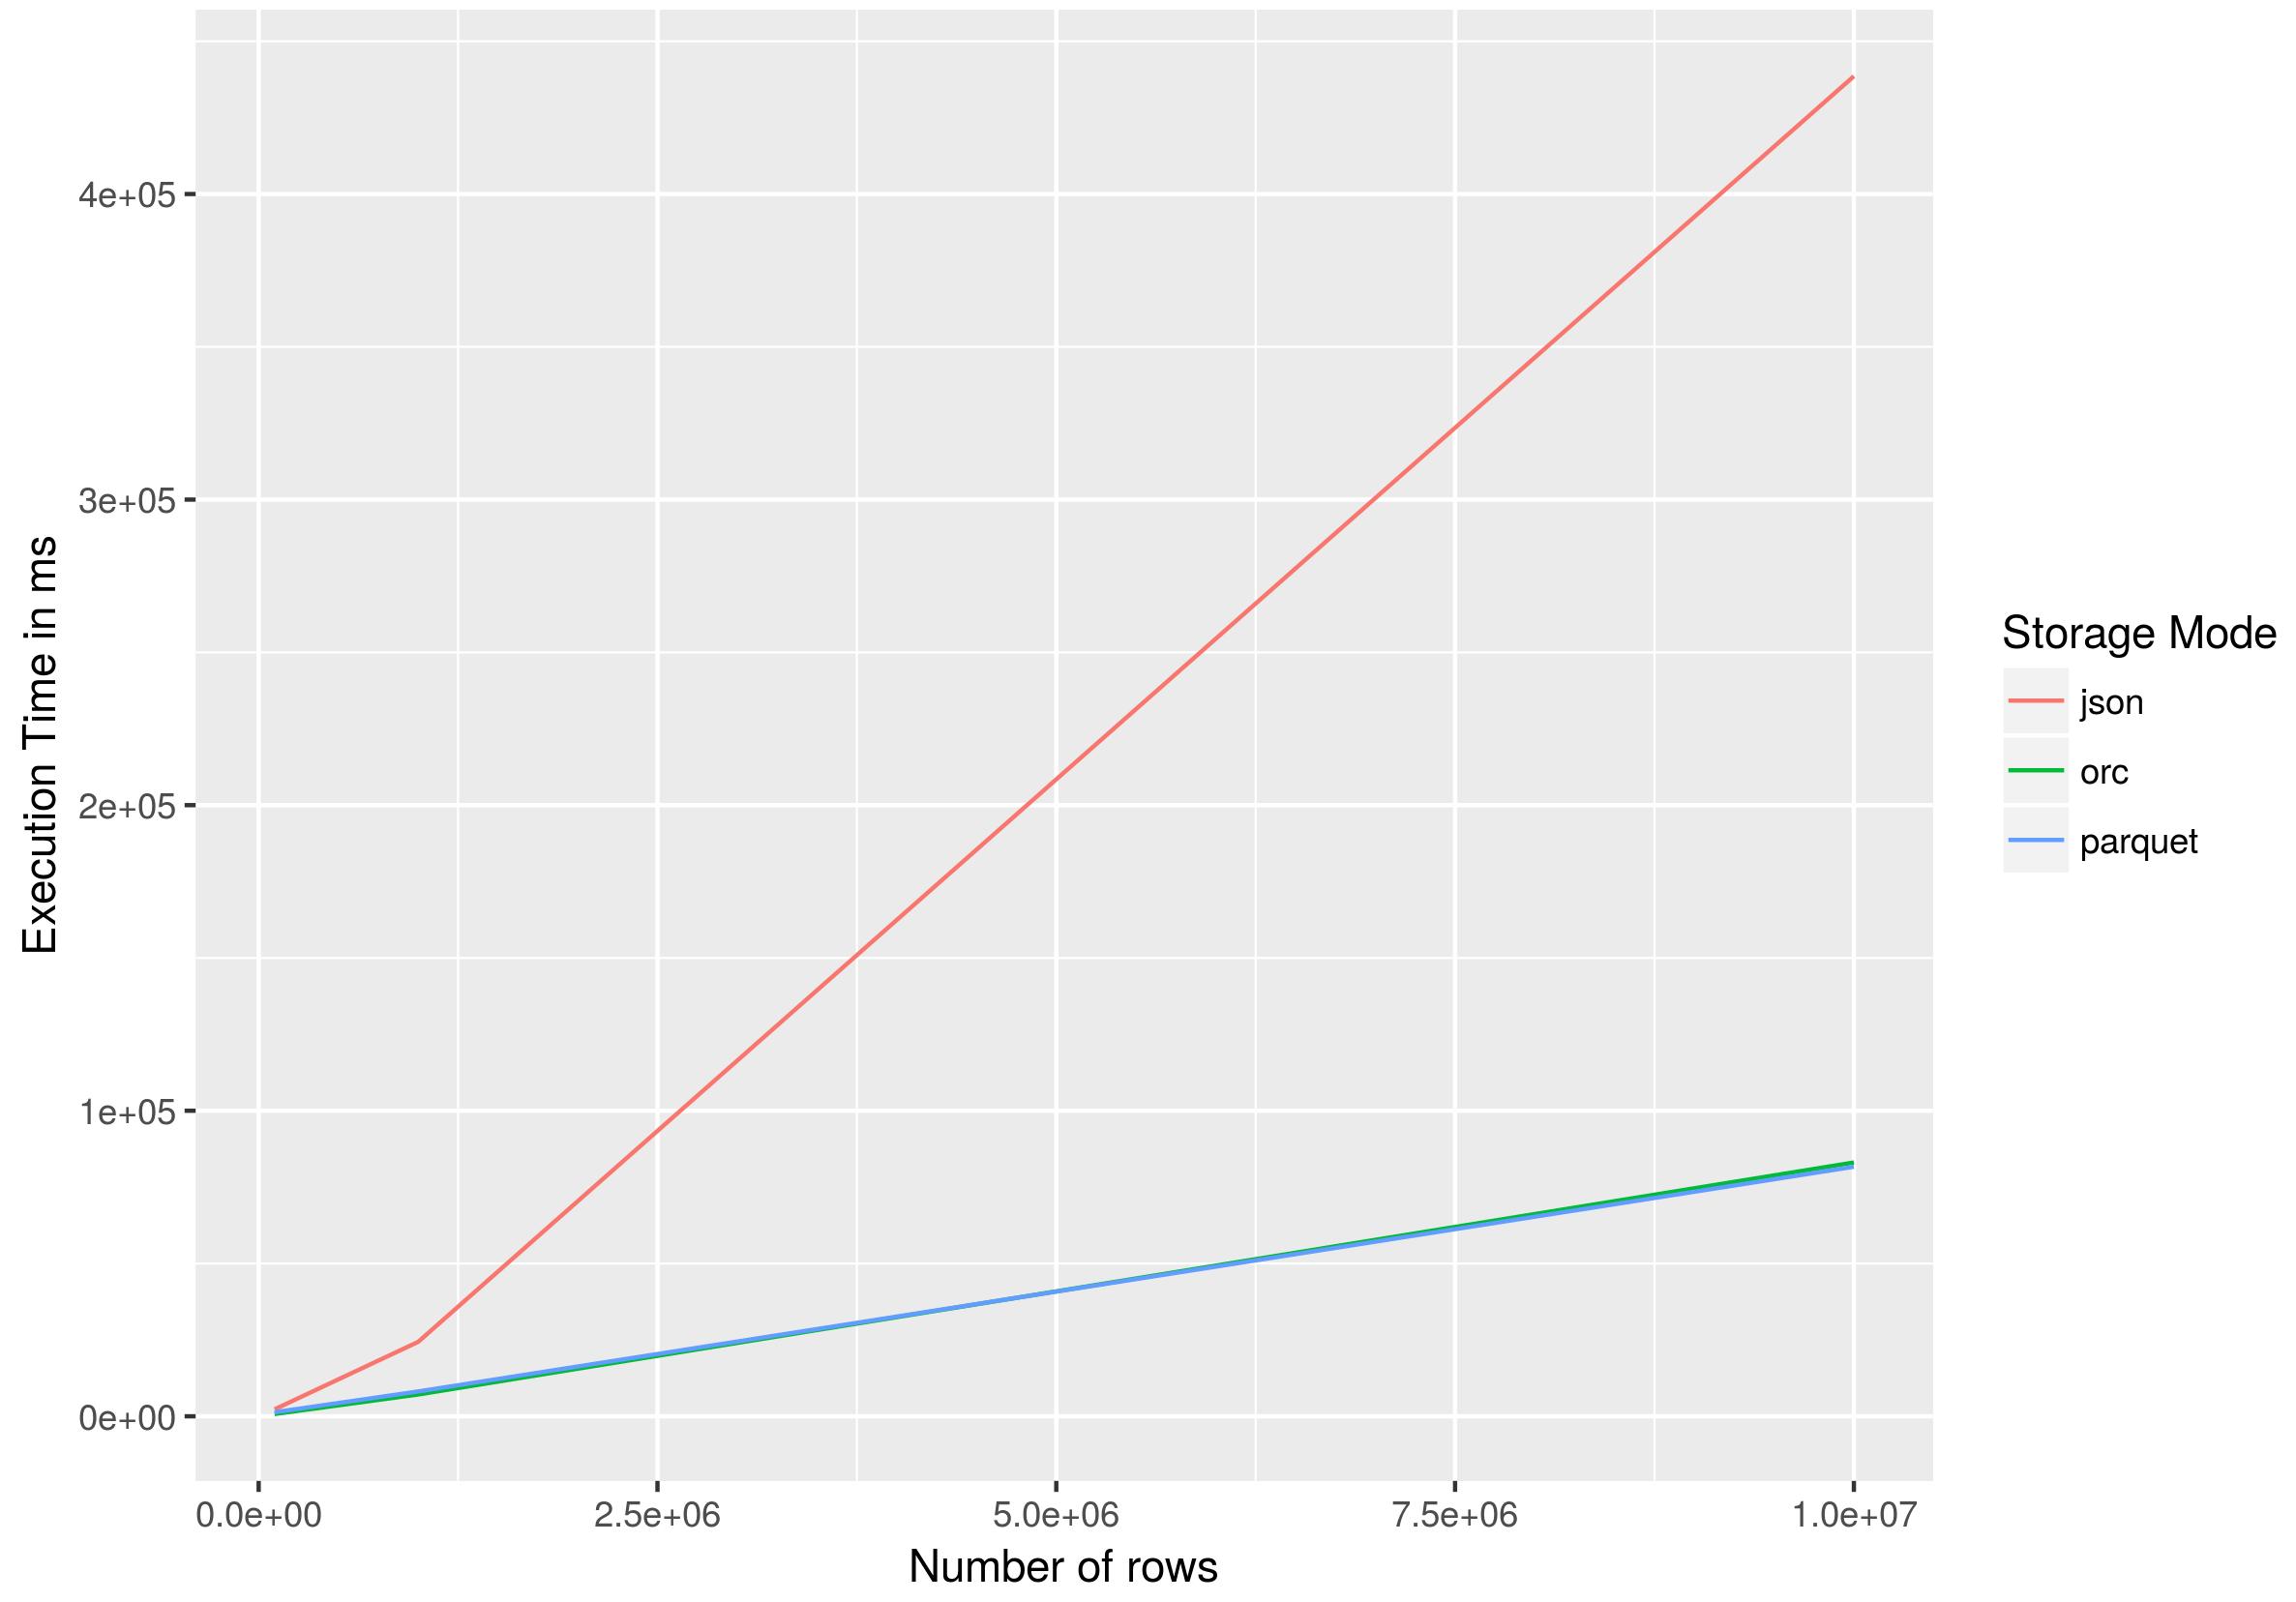
\includegraphics[width=0.75\textwidth]{query-two.png}
\label{fig:query-two}
\end{figure}

As expected, execution time for Parquet is grows linear with the number of rows but the gradient is lower.

\newpage


\section{Lessons Learned} \label{sec:lessons_learned}

\subsection{Tools and Frameworks}
In the beginning, I had trouble figuring out how to use Parquet.
The official Website does not provide any information whatsoever on how to actually use Parquet.
Thankfully, I had worked with Spark in the Context of my Bachelor's Thesis on $ADAM_{pro}$\footnote{https://github.com/vitrivr/ADAMpro} which uses parquet to store data.

Using Scala was an easy choice given that it is the language of choice for Spark.
Utilizing Parquet together with spark is extremely simple.
The basic abstraction of Spark for Data, \textit{Dataframes}, contain write-methods for each storage method used in the benchmark and it requires no setup at all to use parquet together with Spark.
To illustrate, consider the difference between writing data in JSON and writing data in Parquet in Scala-Code.

\renewcommand{\lstlistingname}{Code}

\begin{lstlisting}[language=Scala,caption=Saving a Dataframe with Parquet, label=amb, captionpos=b]
def write(filename: String, df: DataFrame) = {
  df.write.mode(SaveMode.Overwrite).parquet(filename)
}
\end{lstlisting}

When writing a Dataframe to JSON, you simply change the storage-format from parquet to JSON.

\begin{lstlisting}[language=Scala,caption=Saving a Dataframe with JSON, label=amb, captionpos=b]
def write(filename: String, df: DataFrame) = {
  df.write.mode(SaveMode.Overwrite).json(filename)
}
\end{lstlisting}

For reading, the code is similar:

\begin{lstlisting}[language=Scala,caption=Reading a Dataframe with Parquet, label=amb, captionpos=b]
def read(filename: String): DataFrame = {
  sparkSession.read.parquet(filename)
}
\end{lstlisting}

And Spark takes care of the rest.

\subsection{Results}
The main takeaway for me was that there is no reason at all to use JSON or CSV to store large amounts of data when using spark.
Parquet not only saves massive amount of storage space, but also enables faster querying.
I was surprised that ORC held up so well.
If I were to use spark on a massive scale, both ORC and Parquet would warrant taking a closer look.
The performed benchmarks were only a start.
For both ORC and Parquet there exist different compression schemes and different configuration options which have to be tuned for a particular use-case.


% Unfortunetly you cannot use a bibliography generated by BibTeX as a .bbl file.
%
% Use 
%\bibliographystyle{IEEEtran}
% and
%\bibliography{IEEEabrv,../bib/paper} % argument is your BibTeX string definitions and bibliography database(s)
% to generate a .bbl file and copy manually the resultant .bbl file content
% into the thebibliography environment.
% Set second argument of \begin to the number of references (used to reserve space for the reference number labels box).
\begin{thebibliography}{1}

\bibitem{IEEEhowto:kopka}
H.~Kopka and P.~W. Daly, \emph{A Guide to \LaTeX}, 3rd~ed.\hskip 1em plus
  0.5em minus 0.4em\relax Harlow, England: Addison-Wesley, 1999.

\end{thebibliography}
